\documentclass[]{standalone}

\usepackage{tikz}
\usetikzlibrary{calc}
\begin{document}
	\pagestyle{empty}
	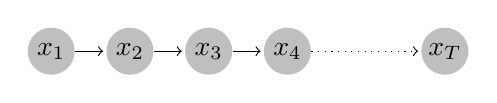
\begin{tikzpicture}[shorten >=1pt,->]
	\tikzstyle{vertex}=[circle,fill=black!25,minimum size=17pt,inner sep=0pt]
	
	\foreach \name/\x in {x_1/1, x_2/2, x_3/3, x_4/4, x_T/6}
	\node[vertex] (G-\name) at (\x,0) {$\name$};
	

	
	\foreach \from/\to in {x_1/x_2,x_2/x_3,x_3/x_4}
	\draw (G-\from) -- (G-\to);
	

	\foreach \from/\to in {x_4/x_T}
	\draw[dotted]  (G-\from) -- (G-\to);
	

	\end{tikzpicture}
	
\end{document}